\section{Ausgangskennlinienfeld}
\subsection{Experimentelle Durchf\"uhrung}
In dem letzten Versuch wird das Ausgangskennlinienfeld, I$_C$ $=$ f(U$_{CE}$) in Abh\"angigkeit des Parameters I$_B$, des NPN-Transistors BC 547C aufgenommen. Aus den Kennlinien wird anschlie\ss end der Kleinsignalwiderstand r$_{CE}$ sowie die Early-Spannung U$_A$ ermittelt.
\begin{figure}[!h]
\begin{center}
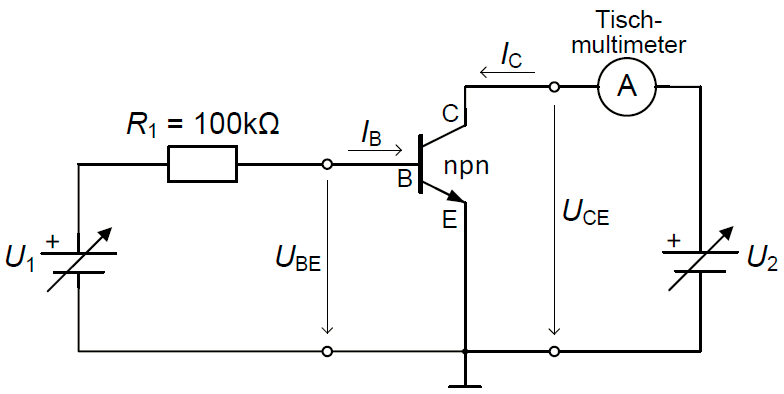
\includegraphics[width=0.8\textwidth]{ausgangsKennlinie}
\caption{Der Versuchsaufbau zur Bestimmung des Ausgangskennlinienfeld des Transistors}
\end{center}
\end{figure}
\subsection{Ergebnisse und Diskussion}
In Tabelle 3 ist der Kollektorstrom in Abh\"angigkeit zu der Kollektorbasisspannung angegeben. 
\begin{figure}[!h]
\begin{center}
\textbf{Tabelle 3: Aufgenommene Messwerte von I$_C$ in Abh\"angigkeit von U$_{CE}$  } \\[0.2cm]
%\caption{}
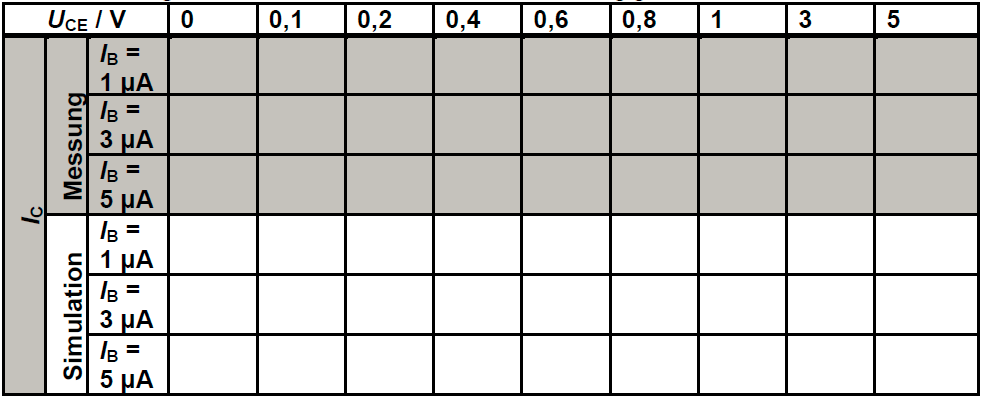
\includegraphics[width=0.8\textwidth]{ergebnissVersuch3}
\end{center}
\end{figure}
\begin{figure}[h]
\begin{center}
\vspace{8cm}
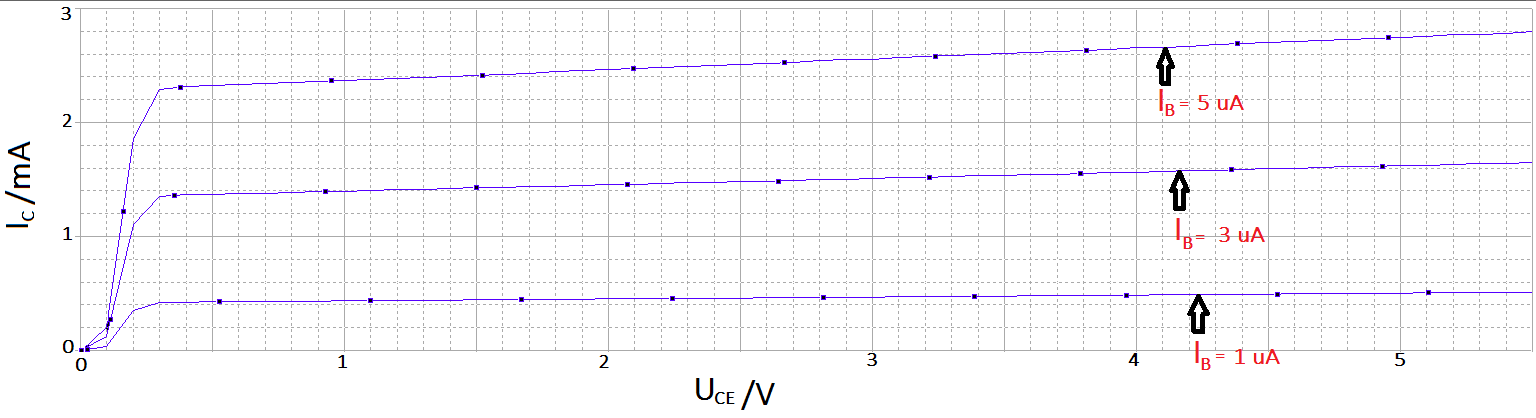
\includegraphics[width=1\textwidth]{Versuch3AllinOne}
\caption{Graphische Darstellung der simulierten Ergebnisse}
\end{center}
Das Ausgangkennlinienfeld stellt die Abh\"angigkeit des Kollektorstroms I$_C$ von der Kollektor-Emitterspannung U$_{CE}$ bei ausgew\"ahlten Basissteuerstr\"omen I$_B$ dar. \\
Der Kleinsignalwiderstand wird wie folgt definiert \\
\begin{equation*}
\text{\text{r$_{CE}$}} = \frac{\Delta U_{CE}}{\Delta I_C}
\end{equation*}
Wir w\"ahlen die Arbeitspunkt  bei einer Spannung U$_{CE}$ $=$ $\frac{\text{U$_{CC}$}}{2}$
\begin{center} 
\begin{tabular}{|l|l|l|}
\hline
Messreihe & r$_{{CE}_{\textbf{Simulation}}}$/$mV$ & r$_{{CE}_{\textbf{Messung}}}$/$mV$\\
\hline
I$_{B_1} = 1~uA$ &  &  \\
\hline
I$_{B_2} = 3~uA$ &  &  \\
\hline
I$_{B_3} = 5~uA$ &  &  \\
\hline
\end{tabular}
\end{center}
Die Early-Spannung U$_A$ l\"asst sich aus folgender Formel herleiten
\begin{equation*}
\text{\textbf{r$_{CE}$}} = \frac{\text{U$_A$}}{\text{I$_C$}} \Rightarrow 
\text{\textbf{\text{U$_A$}}} = \text{r$_{CE}$} \cdot \text{I$_C$}
\end{equation*}
\begin{center}
\begin{tabular}{|l|l|l|}
\hline
Messreihe & U$_{A_{\textbf{Simulation}}}$ & U$_{{A}_{\textbf{Messung}}}$\\
\hline
U$_{A_1}$  &  &  \\
\hline
\end{tabular}
\end{center}
\newpage
Die Early-Spannung soll m\"oglichst gro\ss  sein U$_A$ $\rightarrow$ $\infty$, also w\"are der Transistor eine ideale Stromquelle
 d.h bei der Abbildung (6) wird der Strom I$_C$ so gut wie konstant.  
\end{figure}



